

\item Two identical uniform discs roll without slipping on two different surfaces AB and CD (see figure) starting at A and C with linear speeds $v_1$ and $v_2$, respectively, and always remain in contact with the surfaces. If they reach B and D with the same linear speed and $v_1 = 3$ m/s, then $v_2$ in m/s is (g = 10 m/s\textsuperscript{2})

\begin{center}
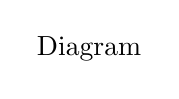
\begin{tikzpicture}
\node {Diagram};
\end{tikzpicture}
\end{center}

